\documentclass[11pt,letterpaper]{report}

\usepackage[letterpaper,margin=1in]{geometry}
\usepackage[T1]{fontenc}
\usepackage{lmodern}
\usepackage{graphicx}
\usepackage{tikz}
\usetikzlibrary{positioning,calc}
\usepackage{listings}
\usepackage{xcolor}
\usepackage{booktabs}
\usepackage{enumitem}
\usepackage{caption}
\usepackage[hidelinks]{hyperref}

\captionsetup{font=small,labelfont=bf}
\lstset{
  basicstyle=\ttfamily\small,
  breaklines=true,
  columns=fullflexible,
  keepspaces=true,
  frame=none,
  aboveskip=0.8em,
  belowskip=0.8em,
  xleftmargin=1.2em
}
\setlist[itemize]{topsep=0.3em,itemsep=0.15em}
\setlist[enumerate]{topsep=0.3em,itemsep=0.15em}

\newcommand{\note}[1]{\par\medskip\noindent\textbf{Note:} #1\par}
\newcommand{\code}[1]{\texttt{#1}}

\begin{document}

% ---------------------------------------------------------------------------
% Title page
% ---------------------------------------------------------------------------
\begin{titlepage}
  \centering
  \vspace*{0.4cm}
  
\includegraphics[width=0.82\textwidth]{figures/upc-fib.png}\par
  \vspace{3.6cm}
  {\Huge\bfseries SRv6 laboratory session\par}
  \vspace{0.45cm}
  {\Large CNANM Laboratory\par}
  \vspace{0.25cm}
  {\large Segment Routing over IPv6 with Mininet and FRR\par}
  \vfill
  {\large Joel González Jiménez\par}
  \vspace{0.25cm}
  {\large November 2026\par}
  \vspace*{0.5cm}
\end{titlepage}

\pagenumbering{arabic}
\tableofcontents
\clearpage

% ---------------------------------------------------------------------------
\chapter{SRv6 in a nutshell}
% ---------------------------------------------------------------------------

\section{Segment Routing over IPv6}

Segment Routing over IPv6 (SRv6) implements source routing on an IPv6 data
plane.  The ingress router encapsulates the original packet inside an outer
IPv6 header and, when necessary, adds a Segment Routing Header (SRH).  The SRH
contains an ordered list of \emph{segments}; each segment is an IPv6 address
called a \emph{Segment Identifier} (SID).  Every SRv6 router that receives a
packet whose outer destination is one of its local SIDs executes the behavior
associated with that SID and, depending on the behavior, forwards the packet
to the next segment.

Because the segment list is carried in the packet, the ingress can choose a
path that differs from the one the IGP would select.  This is the property that
makes SRv6 useful for traffic engineering and service chaining.

\section{Segment identifiers and behaviors}

A SID is normally an IPv6 address inside a \emph{locator} advertised by the
router that owns it.  The behavior attached to a local SID determines what the
router does with the packet.  Table~\ref{tab:behaviors} summarizes the
behaviors used in this laboratory.

\begin{table}[htbp]
  \centering
  \caption{SRv6 behaviors used in the laboratory.}
  \label{tab:behaviors}
  \begin{tabular}{@{}lll@{}}
    \toprule
    Behavior & Action & Typical role \\
    \midrule
    Encap        & Add an outer IPv6 header and an SRH              & Ingress \\
    \texttt{End} & Pop the local SID and forward to the next segment & Transit \\
    \texttt{End.X} & Pop the SID and forward to a specific neighbor  & Transit \\
    \texttt{End.DX6} & Decapsulate and deliver to an IPv6 nexthop  & Egress edge \\
    \bottomrule
  \end{tabular}
\end{table}

The first segment in the list is processed first.  For example, a list
\code{[SID$_A$, SID$_B$]} sends the packet first to the router that owns
\code{SID$_A$}; after that behavior runs, the packet continues toward
\code{SID$_B$}.  The last segment normally delivers the packet to the
destination or hands it to a routing table that knows how to reach it.

\section{Encapsulation and the SRH}

In \emph{encap} mode, the ingress prepends a new IPv6 header and an SRH to the
original packet; the original packet is carried as the payload
(Figure~\ref{fig:encap}).  In \emph{inline} mode the SRH is inserted into the
existing packet instead of adding an outer header.  This laboratory uses
encapsulation mode.

\begin{figure}[htbp]
  \centering
  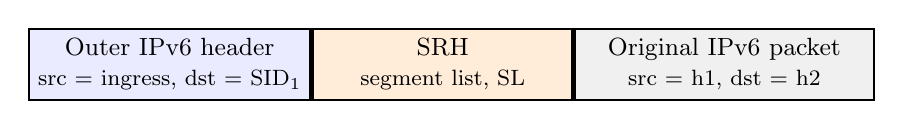
\begin{tikzpicture}[
      pkt/.style={draw,thick,minimum height=9mm,align=center,font=\small},
      node distance=0pt
    ]
    \node[pkt,fill=blue!8,minimum width=3.3cm] (outer)
      {Outer IPv6 header\\ \footnotesize src = ingress, dst = SID$_1$};
    \node[pkt,fill=orange!15,minimum width=3.3cm,right=0pt of outer] (srh)
      {SRH\\ \footnotesize segment list, SL};
    \node[pkt,fill=gray!12,minimum width=3.8cm,right=0pt of srh] (inner)
      {Original IPv6 packet\\ \footnotesize src = h1, dst = h2};
  \end{tikzpicture}
  \caption{Encapsulation mode: the ingress adds an outer IPv6 header and an
  SRH.  The original packet is carried unchanged inside.}
  \label{fig:encap}
\end{figure}

% ---------------------------------------------------------------------------
\chapter{Laboratory environment}
% ---------------------------------------------------------------------------

\section{Prerequisites}

The laboratory runs on Linux with Mininet, FRR and the project's Python
virtual environment.  From the repository root, run the setup and preflight
commands once:

\begin{lstlisting}
./scripts/setup.sh
make doctor
make check ARGS=topologies/srv6_lab1.yaml
\end{lstlisting}

The last command parses and validates the initial topology without starting the
lab.

\section{Starting the laboratory}

The initial topology for this session is \code{topologies/srv6\_lab1.yaml}.
Start the lab with:

\begin{lstlisting}
make run ARGS="topologies/srv6_lab1.yaml"
\end{lstlisting}

To stop the lab, type \code{exit} at the \code{mininet>} prompt.  If a crash or
an interrupt leaves namespaces or daemons behind, clean them with:

\begin{lstlisting}
make clean
\end{lstlisting}

\note{Keep one copy of the topology file per exercise (for example, a file
named \code{step1.yaml}).  Restart the lab after every topology change so
that the controller reloads the baseline and the daemons re-read their
configuration.}

\section{Mininet command line}

The Mininet CLI accepts commands on the emulated hosts and routers.  The most
useful ones are:

\begin{itemize}
  \item \code{nodes}: list all nodes in the network.
  \item \code{dump}: show addresses, interfaces and PIDs.
  \item \code{<node> <command>}: run a command on a node, for example
        \code{h1 ping -6 -c 3 <address>} or \code{r1 ip -6 route}.
  \item \code{pingall}: ping every pair of hosts.
  \item \code{exit}: stop the network.
\end{itemize}

Useful verification commands inside the nodes include \code{ip -6 addr},
\code{ip -6 route}, \code{traceroute -6} and
\code{tcpdump -ni any -vv ip6 proto 43} (the last one shows SRH packets).

\section{Naming and addressing conventions}

The exercises follow these conventions:

\begin{itemize}
  \item Routers are named \code{r<number>}, hosts \code{h<number>}, and
        SRv6-enabled routers \code{sr<number>}.
  \item Every router has a loopback address
        \code{2001:db8:<number>::1/64}.
  \item Local SIDs must belong to the router's loopback locator; for example,
        a SID on \code{r4} can be \code{2001:db8:4::10}.
  \item Links are bidirectional.
  \item Host addresses are assigned by ipmininet.  Read them with
        \code{<host> ip -6 addr} before testing connectivity.
\end{itemize}

\section{Initial topology}

Figure~\ref{fig:initial} shows the starting topology.  It is intentionally
small: the exercises add routers, links and SRv6 state step by step.

\begin{figure}[htbp]
  \centering
  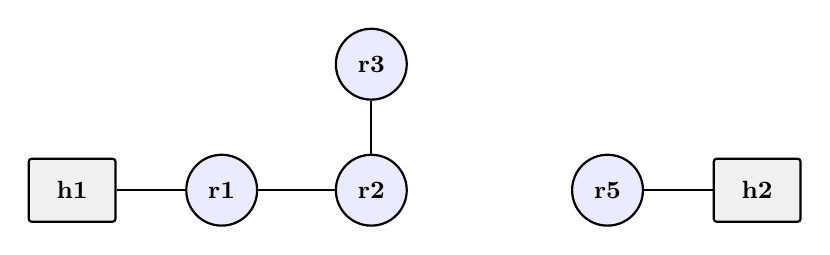
\begin{tikzpicture}[
      router/.style={circle,draw,thick,minimum size=9mm,fill=blue!8,
                     font=\small\bfseries},
      host/.style={rectangle,draw,thick,rounded corners=1pt,
                   minimum width=11mm,minimum height=8mm,fill=gray!12,
                   font=\small\bfseries},
      link/.style={thick}
    ]
    \node[host]   (h1) at (0,0)    {h1};
    \node[router] (r1) at (1.9,0)  {r1};
    \node[router] (r2) at (3.8,0)  {r2};
    \node[router] (r3) at (3.8,1.6){r3};
    \node[router] (r5) at (6.8,0)  {r5};
    \node[host]   (h2) at (8.7,0)  {h2};
    \draw[link] (h1) -- (r1);
    \draw[link] (r1) -- (r2);
    \draw[link] (r2) -- (r3);
    \draw[link] (r5) -- (h2);
  \end{tikzpicture}
  \caption{Initial topology defined in \code{topologies/srv6\_lab1.yaml}.
  All links are bidirectional.}
  \label{fig:initial}
\end{figure}

% ---------------------------------------------------------------------------
\chapter{Laboratory exercises}
% ---------------------------------------------------------------------------

Work on a copy of the topology file for each exercise and restart the lab
after every change. 

\section{Exercise 1: basic reachability}

\begin{enumerate}
  \item Start the lab with the initial topology.
  \item Test connectivity between \code{h1} and \code{h2}.  Record the result
        and explain it from the topology.
  \item Add a router \code{r4} with loopback \code{2001:db8:4::1/64} and links
        \code{r2--r4} and \code{r4--r5}.  Restart the lab and repeat the test.
  \item Inspect the forwarding path with \code{traceroute -6} or
        \code{ip -6 route} on the routers.
\end{enumerate}

\paragraph{Q1.} Does the initial topology provide connectivity between
\code{h1} and \code{h2}?

\paragraph{Q2.} After adding \code{r4}, does the traffic between the hosts go
through every router?  Which path is used, and why?

\section{Exercise 2: SRv6 ingress and egress}

\begin{enumerate}
  \item Upgrade \code{r1} and \code{r5} to SRv6 routers.  Follow the naming
        convention and call them \code{sr1} and \code{sr2}.  Give each router a
        loopback locator and at least one local SID.  Configure \code{sr1} as
        the ingress and \code{sr2} as the egress for the \code{h1 -> h2}
        direction.
  \item Add a router \code{r6} that connects \code{sr1} to \code{h2}, and a
        router \code{r7} that connects \code{sr2} to \code{h1}.  Give both new
        routers a loopback address.
  \item Test both directions, \code{h1 -> h2} and \code{h2 -> h1}.  Record the
        paths and the segment lists used by the policies.
  \item Make \code{sr1} and \code{sr2} both ingress and egress routers.  Repeat
        the tests and compare the two directions.
        
\end{enumerate}

\paragraph{Q3.} Do the flows follow the shortest path in each direction?

\paragraph{Q4.} Which routers are unused in each of the configurations above?

\paragraph{Q5.} What changes when \code{sr1} and \code{sr2} are both ingress
and egress routers?  Why is the return direction affected?

\section{Exercise 3: forcing a detour through r3}

Add a router \code{r9} with loopback \code{2001:db8:9::1/64} and links
\code{r3--r9} and \code{r9--r4}. \\

\noindent How can the traffic between \code{h1} and \code{h2} be made to pass through
\code{r3}? You may change router roles, local SIDs, policy segment lists.


\paragraph{Q7.} Which router or routers did you modify, and why?

\paragraph{Q8.} What is the resulting path for \code{h1 -> h2} and for
\code{h2 -> h1}?  Does the detour apply symmetrically?

\clearpage

% ---------------------------------------------------------------------------
\appendix
\chapter{Troubleshooting and cleanup}
% ---------------------------------------------------------------------------

\begin{itemize}
  \item If the lab does not start, run \code{make doctor} and check the
        prerequisites (Mininet, FRR, \code{.venv} and SRv6 support).
  \item If a policy reports an error immediately after startup, OSPFv3 may not
        have converged yet.  Wait a few seconds and run
        \code{./scripts/srctl.sh reconcile}.
  \item Use \code{./scripts/srctl.sh diff -f <file>} before
        \code{apply}; it shows the planned actions without changing the data
        plane.
  \item After a crash or an interrupt, run \code{make clean} to remove the
        Mininet namespaces and leftover FRR processes.
  \item To observe SRv6 packets, run
        \code{tcpdump -ni any -vv ip6 proto 43} on a router and send traffic
        that matches a policy.
\end{itemize}

\note{Do not modify the topology files supplied for the session; keep your
exercise topologies in separate files.}

\end{document}
